\documentclass[12pt, a4paper]{report}

% -------------------------------------------------------------------
% PACKAGES
% -------------------------------------------------------------------
\usepackage[utf8]{inputenc}
\usepackage[T1]{fontenc}
\usepackage{amsmath, amsfonts}
\usepackage{graphicx}
\usepackage[margin=1in]{geometry}
\usepackage{hyperref}
\usepackage{listings}
\usepackage{float}
\usepackage{longtable}
\usepackage{caption}
\usepackage{subcaption}
\usepackage{fancyhdr}
\usepackage{xcolor}

% TikZ for Diagrams
\usepackage{tikz}
\usetikzlibrary{shapes.geometric, arrows, positioning, calc}

% -------------------------------------------------------------------
% CONFIGURATION
% -------------------------------------------------------------------

% Hyperlink Setup
\hypersetup{
    colorlinks=true,
    linkcolor=black,
    filecolor=magenta,      
    urlcolor=blue,
    pdftitle={University Management System Technical Report},
}

% Java Code Listing Style
\definecolor{codegreen}{rgb}{0,0.6,0}
\definecolor{codegray}{rgb}{0.5,0.5,0.5}
\definecolor{codepurple}{rgb}{0.58,0,0.82}
\definecolor{backcolour}{rgb}{0.96,0.96,0.96}

\lstset{
    language=Java,
    backgroundcolor=\color{backcolour},   
    commentstyle=\color{codegreen},
    keywordstyle=\color{purple}\bfseries,
    numberstyle=\tiny\color{codegray},
    stringstyle=\color{blue},
    basicstyle=\ttfamily\footnotesize,
    breakatwhitespace=false,         
    breaklines=true,                 
    captionpos=b,                    
    keepspaces=true,                 
    numbers=left,                    
    numbersep=5pt,                  
    showspaces=false,                
    showstringspaces=false,
    showtabs=false,                  
    tabsize=4,
    frame=lines
}

% Flowchart Styles
\tikzstyle{startstop} = [rectangle, rounded corners, minimum width=3cm, minimum height=1cm,text centered, draw=black, fill=red!30]
\tikzstyle{io} = [trapezium, trapezium left angle=70, trapezium right angle=110, minimum width=3cm, minimum height=1cm, text centered, draw=black, fill=blue!30]
\tikzstyle{process} = [rectangle, minimum width=3cm, minimum height=1cm, text centered, draw=black, fill=orange!30]
\tikzstyle{decision} = [diamond, minimum width=3cm, minimum height=1cm, text centered, draw=black, fill=green!30]
\tikzstyle{arrow} = [thick,->,>=stealth]

% Class Diagram Styles
\tikzstyle{class} = [rectangle, draw=black, fill=yellow!20, minimum width=4cm, align=center]

% Header and Footer
\pagestyle{fancy}
\fancyhf{}
\rhead{UMS Technical Report}
\lhead{\leftmark}
\cfoot{\thepage}

\begin{document}

% -------------------------------------------------------------------
% TITLE PAGE
% -------------------------------------------------------------------
\begin{titlepage}
    \begin{center}
        \vspace*{1cm}
        
        \Huge
        \textbf{University Management System}
        
        \vspace{0.5cm}
        \Large
        \textit{A Software Engineering Technical Report}
        
        \vspace{2cm}
        
        \textbf{Submitted by:}
        
        \vspace{0.5cm}
        \Large
        \textbf{[Your Name Here]} \\
        \large
        [Student ID Here]
        
        \vspace{2cm}
        
        \includegraphics[width=0.3\textwidth]{example-image-a} % Placeholder for Logo
        
        \vspace{2cm}
        
        \Large
        \textbf{Department of Computer Science} \\
        \textbf{[University Name Here]} \\
        [Date of Submission]
        
    \end{center}
\end{titlepage}

% -------------------------------------------------------------------
% FRONT MATTER
% -------------------------------------------------------------------
\pagenumbering{roman}

\chapter*{Abstract}
\addcontentsline{toc}{chapter}{Abstract}
The University Management System (UMS) is a comprehensive Java-based application designed to streamline administrative and academic processes. Leveraging Object-Oriented Programming (OOP) principles, the system provides a robust platform for Student Registration, Course Enrollment, Faculty Grading, and Fee Management.
\par
The application is built using Java SE for core logic, Java Swing/JavaFX for the Graphical User Interface (GUI), and MySQL for persistent data storage. This report details the system architecture, design patterns, and implementation strategies used to ensure scalability, security, and maintainability.

\tableofcontents
\listoffigures
\listoftables

\newpage
\pagenumbering{arabic}

% -------------------------------------------------------------------
% CHAPTER 1: INTRODUCTION
% -------------------------------------------------------------------
\chapter{Introduction}

\section{Problem Statement}
Managing university operations manually is error-prone and inefficient. Issues include:
\begin{itemize}
    \item \textbf{Data Redundancy:} Duplicate records across different departments.
    \item \textbf{Slow Processing:} Manual fee calculation and grade entry take weeks.
    \item \textbf{Lack of Integrity:} No proper validation for prerequisites during course registration.
\end{itemize}

\section{Project Objectives}
The primary objective is to develop a UMS that:
\begin{enumerate}
    \item Automates the **Student Registration** process.
    \item Provides a secure **Admin Dashboard** for managing system users.
    \item Enables **Faculty Grading** with automatic GPA calculation.
    \item Manages **Fee Payments** and generates receipts.
    \item Demonstrates core **OOP Principals** (Inheritance, Polymorphism) in action.
\end{enumerate}

% -------------------------------------------------------------------
% CHAPTER 2: SYSTEM DESIGN
% -------------------------------------------------------------------
\chapter{System Design}

\section{UML Class Diagram}
The system uses a hierarchical class structure to maximize code reuse. The diagram below illustrates the inheritance relationship between the base `User` class and its derived classes.

\begin{figure}[H]
    \centering
    \begin{tikzpicture}[node distance=2cm]
        % Nodes
        \node (User) [class, rectangle split, rectangle split parts=2] {
            \textbf{User} (Abstract)
            \nodepart{second}
            - id: int \\ - name: String \\ - email: String \\ + login(): boolean
        };
        
        \node (Student) [class, rectangle split, rectangle split parts=2, below left=of User, xshift=-0.5cm] {
            \textbf{Student}
            \nodepart{second}
            - gpa: double \\ - major: String \\ + registerCourse() \\ + viewGrades()
        };
        
        \node (Faculty) [class, rectangle split, rectangle split parts=2, below right=of User, xshift=0.5cm] {
            \textbf{Faculty}
            \nodepart{second}
            - department: String \\ - salary: double \\ + addGrade() \\ + viewSchedule()
        };
        
        \node (Admin) [class, rectangle split, rectangle split parts=2, right=of Faculty, xshift=1cm] {
            \textbf{Admin}
            \nodepart{second}
            - adminLevel: int \\ + addUser() \\ + manageFees()
        };
        
        % Arrows
        \draw [arrow] (User) -- (Student);
        \draw [arrow] (User) -- (Faculty);
        \draw [arrow] (User) -- (Admin);
        
    \end{tikzpicture}
    \caption{UML Class Diagram showing Inheritance Hierarchy}
    \label{fig:class_diagram}
\end{figure}

\section{Process Flowcharts}

\subsection{Login Process}
The following flowchart details the authentication logic implemented in the `LoginController`.

\begin{figure}[H]
    \centering
    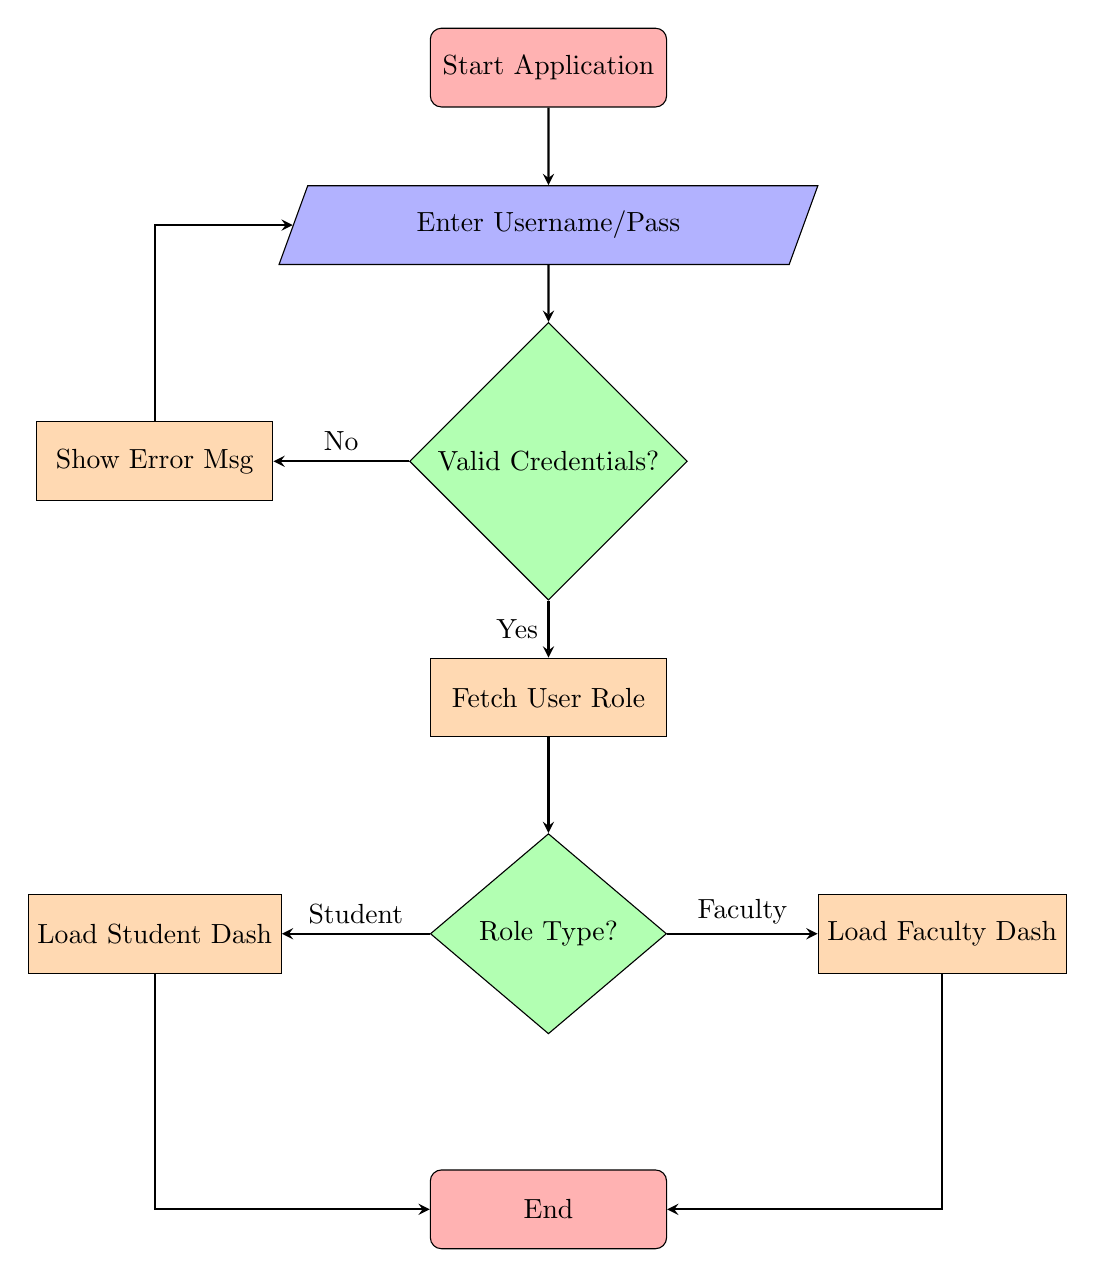
\begin{tikzpicture}[node distance=2cm]
        \node (start) [startstop] {Start Application};
        \node (in1) [io, below of=start] {Enter Username/Pass};
        \node (dec1) [decision, below of=in1, yshift=-1cm] {Valid Credentials?};
        \node (proc1) [process, left of=dec1, xshift=-3cm] {Show Error Msg};
        \node (proc2) [process, below of=dec1, yshift=-1cm] {Fetch User Role};
        \node (dec2) [decision, below of=proc2, yshift=-1cm] {Role Type?};
        \node (stud) [process, left of=dec2, xshift=-3cm] {Load Student Dash};
        \node (fac) [process, right of=dec2, xshift=3cm] {Load Faculty Dash};
        \node (stop) [startstop, below of=dec2, yshift=-1.5cm] {End};

        \draw [arrow] (start) -- (in1);
        \draw [arrow] (in1) -- (dec1);
        \draw [arrow] (dec1) -- node[anchor=south] {No} (proc1);
        \draw [arrow] (proc1) |- (in1);
        \draw [arrow] (dec1) -- node[anchor=east] {Yes} (proc2);
        \draw [arrow] (proc2) -- (dec2);
        \draw [arrow] (dec2) -- node[anchor=south] {Student} (stud);
        \draw [arrow] (dec2) -- node[anchor=south] {Faculty} (fac);
        \draw [arrow] (stud) |- (stop);
        \draw [arrow] (fac) |- (stop);
    \end{tikzpicture}
    \caption{Flowchart: User Login Logic}
    \label{fig:flow_login}
\end{figure}

\subsection{Course Registration Logic}
The registration module ensures students cannot exceed credit limits or join full classes.

\begin{figure}[H]
    \centering
    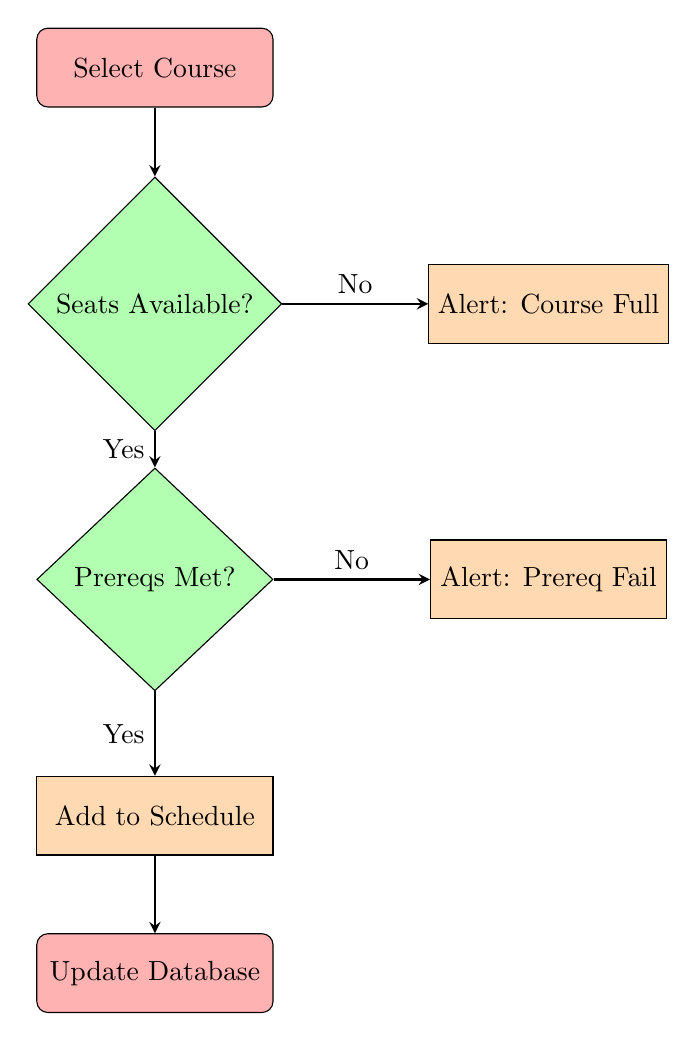
\begin{tikzpicture}[node distance=2cm]
        \node (start) [startstop] {Select Course};
        \node (dec1) [decision, below of=start, yshift=-1cm] {Seats Available?};
        \node (stop1) [process, right of=dec1, xshift=3cm] {Alert: Course Full};
        \node (dec2) [decision, below of=dec1, yshift=-1.5cm] {Prereqs Met?};
        \node (stop2) [process, right of=dec2, xshift=3cm] {Alert: Prereq Fail};
        \node (proc1) [process, below of=dec2, yshift=-1cm] {Add to Schedule};
        \node (end) [startstop, below of=proc1] {Update Database};

        \draw [arrow] (start) -- (dec1);
        \draw [arrow] (dec1) -- node[anchor=south] {No} (stop1);
        \draw [arrow] (dec1) -- node[anchor=east] {Yes} (dec2);
        \draw [arrow] (dec2) -- node[anchor=south] {No} (stop2);
        \draw [arrow] (dec2) -- node[anchor=east] {Yes} (proc1);
        \draw [arrow] (proc1) -- (end);
    \end{tikzpicture}
    \caption{Flowchart: Course Registration Checks}
    \label{fig:flow_reg}
\end{figure}

% -------------------------------------------------------------------
% CHAPTER 3: IMPLEMENTATION DETAILS
% -------------------------------------------------------------------
\chapter{Implementation Details}

\section{OOP Principles in Action}
This project is a practical demonstration of core Object-Oriented Programming concepts.

\subsection{Inheritance}
We utilize the `extends` keyword to create a specialized `User` hierarchy. The `User` class holds common data (ID, Name, Password), while `Student` adds academic specific data (GPA, Major).

\begin{lstlisting}[caption={Inheritance Implementation}]
public abstract class User {
    protected int id;
    protected String username;
    
    public abstract void dashboard(); // Abstract method
}

public class Student extends User {
    private double gpa;
    
    @Override
    public void dashboard() {
        System.out.println("Displaying Student Dashboard...");
    }
}
\end{lstlisting}

\subsection{Polymorphism}
Polymorphism allows the system to treat different user types uniformly. For instance, the `LoginController` validates a user and calls the `dashboard()` method. Depending on whether the object is an instance of `Student` or `Teacher`, the correct dashboard text is displayed.

\subsection{Encapsulation}
All data fields are `private`. Access is restricted to `public` getter and setter methods. This ensures that validation (e.g., checking for negative salary) happens inside the setter before the variable is modified.

\section{Core Modules}

\subsection{Admin Dashboard}
The Admin Dashboard is the central control hub. It allows the administrator to:
\begin{enumerate}
    \item Create new Faculty and Student accounts.
    \item Manage Course Layouts (semesters, credits).
    \item View system-wide logs.
\end{enumerate}

\subsection{Fee Management System}
A critical requirement for the university. The `FeeManager` class handles:
\begin{itemize}
    \item **Tuition Calculation:** Based on credit hours registered ($Cost = Credits \times Rate$).
    \item **Payment Processing:** Updates the `balance` field in the database.
    \item **Receipt Generation:** Prints a text-based receipt for the student.
\end{itemize}

\section{Graphical User Interface (GUI)}
The UI is built using Java Swing. Below are the key screens.

\begin{figure}[H]
    \centering
    % Placeholder for Screenshot
    \fbox{\parbox{10cm}{\centering \vspace{3cm} \textbf{[Screenshot: Student Registration Form]} \vspace{3cm}}}
    \caption{Student Registration Form showing text fields for Name, DOB, and Major selection dropdown.}
    \label{fig:ui_reg}
\end{figure}

\begin{figure}[H]
    \centering
    % Placeholder for Screenshot
    \fbox{\parbox{10cm}{\centering \vspace{3cm} \textbf{[Screenshot: Fee Payment Window]} \vspace{3cm}}}
    \caption{Fee Payment Interface displaying total due and payment history.}
    \label{fig:ui_fee}
\end{figure}

\section{Code Listings}

\subsection{Database Connection (MySQL)}
\begin{lstlisting}[caption={DBConnection.java}]
public class DBConnection {
    public static Connection connect() {
        try {
            Class.forName("com.mysql.cj.jdbc.Driver");
            return DriverManager.getConnection("jdbc:mysql://localhost:3306/ums", "root", "password");
        } catch (Exception e) {
            e.printStackTrace();
            return null;
        }
    }
}
\end{lstlisting}

% -------------------------------------------------------------------
% CHAPTER 4: CONCLUSION
% -------------------------------------------------------------------
\chapter{Conclusion and Future Scope}
The University Management System successfully digitizes the core academic processes. By rigorously applying OOP standards, the system is modular and easy to extend.

\textbf{Future Enhancements:}
\begin{itemize}
    \item **Cloud Integration:** Move from local MySQL to AWS RDS.
    \item **Mobile App:** Develop a Flutter app for students.
    \item **AI Analytics:** Predict student dropout rates based on grades.
\end{itemize}

\end{document}
